% Secciones del juego: historia, cómo jugar, el HUD numerado, puntuación y vidas, consejos.
\sect{5. El juego original}

\textbf{Commando} (en Japón \textit{Senj\=o no \=Okami}, ``el lobo del campo de batalla'') lo publicó Capcom para recreativas en
mayo de 1985. Lo diseñó Tokuro Fujiwara, que a la vez hacía \textit{Ghosts'n Goblins}. Eres \textbf{Super Joe}, un soldado
al que un helicóptero deja solo en territorio enemigo y que tiene que abrirse paso a pie, armado con un fusil y unas pocas
granadas.

Fue una de las recreativas de más éxito de 1985 en Estados Unidos y el Reino Unido, y sus versiones domésticas encabezaron
las listas de ventas aquellas Navidades. Popularizó el juego de disparos a pie con desplazamiento vertical y tuvo muchos
imitadores, como \textit{Ikari Warriors} de SNK. Su continuación fue \textit{Mercs} (1989), y Super Joe volvió en
\textit{Bionic Commando}. Esta versión conserva la recreativa tal como era: sus ocho áreas, sus enemigos, su música y sus
reglas.

\sect{6. Cómo se juega}

Avanzas hacia arriba de la pantalla atravesando las líneas enemigas. Los soldados llegan por todos lados, corren hacia ti y
disparan; otros esperan en trincheras, tras sacos terreros o en búnkeres, y por el camino se suman morteros, jeeps, camiones
y motos.

\begin{itemize}
\item \textbf{Pierdes una vida} si te alcanza una bala, si te toca un soldado o un vehículo, si estalla a tu lado una
explosión (una granada o un proyectil de mortero, también tus propias granadas) o si te metes en el río.
\item \textbf{Las granadas} son tu arma contra lo que el fusil no puede dañar: búnkeres, camiones, morteros y soldados a
cubierto. Una sola granada puede acabar con varios enemigos a la vez, y eso da una bonificación.
\item \textbf{Prisioneros.} De vez en cuando unos guardias llevan a un prisionero por la pantalla. Mata a todos los guardias y
el prisionero queda libre.
\item \textbf{Cajas de granadas} en el suelo: pasa por encima de una para coger 1, 3 o 5 granadas.
\item \textbf{Oficiales.} De vez en cuando un soldado de verde cruza la pantalla corriendo sin disparar: un oficial que huye.
Dispárale y te da 2000 puntos.
\item \textbf{Final de un área.} Al final de cada área la pantalla se detiene ante una puerta. De ella salen soldados; cuando
han salido todos y los has derrotado, Super Joe cruza la puerta y una breve imagen cierra el área.
\item \textbf{Áreas.} Hay cuatro áreas por vuelta; la cuarta termina en una fortaleza, donde te recoge el helicóptero y te
lleva a la siguiente vuelta (áreas 5 a 8). Después del área~8 el juego vuelve a empezar por el área~1, y sigue hasta que
pierdes la última vida. Cada área superada añade una medalla al panel.
\end{itemize}

\begin{figure}[H]
\centering
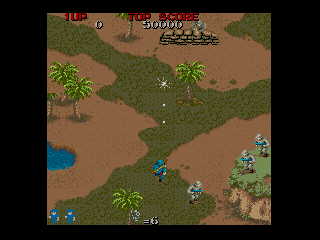
\includegraphics[width=0.48\textwidth]{../img/manual-area1.png}\hfill
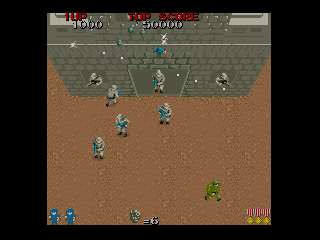
\includegraphics[width=0.48\textwidth]{../img/manual-fortress.png}
\caption{Izquierda: el área 1, con una trinchera de sacos terreros. Derecha: la fortaleza al final del área 4, con sus
soldados saliendo y un oficial de verde huyendo.}
\end{figure}

\clearpage   % the panel heading stays with its picture
\sect{7. El panel de estado (HUD)}

La puntuación está arriba de la pantalla; tus vidas, granadas y medallas, abajo.

\begin{figure}[H]
\centering
\includegraphics[width=0.46\textwidth]{img/hud.png}
\caption{La pantalla de juego y su panel de estado.}
\end{figure}

\begin{tabularx}{\textwidth}{@{}cp{3.6cm}X@{}}
\toprule
\textbf{\tNo} & \textbf{\tElement} & \textbf{\tTellsYou}\\
\midrule
1 & \texttt{1UP} & Tu puntuación.\\
2 & \texttt{TOP SCORE} & La mejor puntuación del ranking (50000 al encender).\\
3 & Vidas & Las vidas que te quedan, además de la que estás jugando.\\
4 & Granadas & Las granadas que te quedan.\\
5 & Medallas & Una medalla por cada área superada.\\
\bottomrule
\end{tabularx}

\sect{8. Puntuación, vidas y récords}

\begin{itemize}
\item \textbf{Vidas.} Empiezas con 3. Ganas una vida extra a los \textbf{10.000} puntos y después cada \textbf{50.000} puntos.
\item \textbf{Al perder una vida} vuelves a empezar desde el último punto por el que pasaste, con al menos 6 granadas. La
partida también empieza con 6 granadas; puedes llevar hasta 99.
\item \begin{minipage}[t]{\linewidth}\textbf{Puntos.}
\begin{center}
\begin{tabular}{@{}lr@{}}
\toprule
Soldado & de 200 a 500\\
Soldado a cubierto & 200\\
Oficial de verde & 2000\\
Guardia de un prisionero & 1000\\
Prisionero liberado & 1000\\
Mortero & 500\\
Búnker (dos granadas) & 500 + 1000\\
Camión / camión con artillero (granada) & 500 / 1000\\
Jeep (siete disparos) & 200 por disparo\\
Caja de granadas & 1000\\
Varios enemigos con una granada (bonificación) & de 200 a 3000\\
Área superada & 5000\\
\bottomrule
\end{tabular}
\end{center}\end{minipage}
\item \textbf{Récords.} Si tu puntuación final está entre las siete mejores, escribes tu nombre: mueve el soldado de abajo a
izquierda y derecha para elegir columna, sube y baja el cursor para elegir fila y dispara a una letra para escribirla. El
punto y el corazón también son letras; el pequeño signo \texttt{RB} borra la última letra y \texttt{ED} termina. Tienes 60
segundos (\texttt{TIMER}). El ranking se conserva hasta que apagas el MSX.
\end{itemize}

\sect{9. Consejos}

\begin{itemize}
\item No te quedes quieto: casi todos los soldados apuntan a donde estás.
\item Guarda granadas para los búnkeres, los morteros y los camiones, y para la puerta del final de cada área, donde salen
muchos soldados juntos.
\item Una granada que pilla a varios soldados da hasta 3000 puntos de bonificación.
\item No dejes escapar a los oficiales de verde: 2000 puntos cada uno.
\item Libera a los prisioneros: 1000 puntos por cada guardia y otros 1000 por el prisionero.
\item Mantente lejos de tus propias granadas y de los proyectiles de mortero: su explosión también te mata a ti.
\end{itemize}
